%_____________________________________________________________________________________________ 
% LATEX Template: Department of Comp/IT BTech Project Reports
% Sample Chapter
% Sun Mar 27 10:25:35 IST 2011
%
% Note: Itemization, enumeration and other things not shown. A sample figure is included.
%_____________________________________________________________________________________________ 

\chapter{Proposed Methodology}
\text{Route alignment optimization is a process to minimize costs involved in road construction and hence optimize the alignments. Our proposed solution is broadly a 3-step procedure involving the following steps:}
\begin{enumerate}
    \item Land Use Land Cover Classification
    \item Weight Assignment and Ranking
    \item  Route alignment Optimization
\end{enumerate}
% \begin{figure}[H]\centering
% 	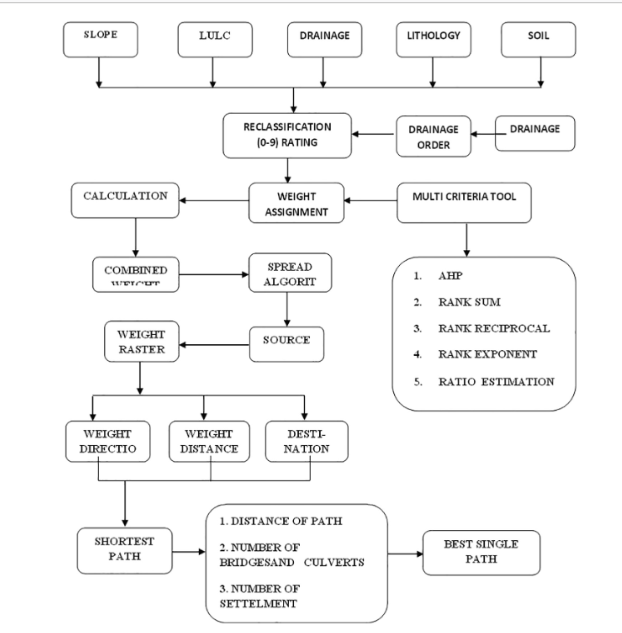
\includegraphics[width=400pt,height=400pt]{steps.png}
% 	\caption{Flowchart for steps performed for Route Alignment Optimization}
% \end{figure}
\section{Study Area }
\text{
Our project involves optimizing the route alignment of the distance between Pune and Mumbai cities of Maharashtra. The present distance of the Pune-Mumbai Expressway is 97.2 km which currently stays overloaded due to traffic and accident prone too. The construction also adversely affected the forest areas, environment and also the communities involved. We aim to optimize the route of Pune-Mumbai expressway and suggest alternative routes using Machine learning and Deep learning based models which would lead to minimized economical, social and environmental costs and enhance utility of the road by making it more safer and connected to other highway networks. For this, we have used the Sentinel-2 image of the Pune-Mumbai region which is then processed in further steps to predict optimized routes to connect the 2 cities. Sentinel-2 images are multi-spectral images consisting of 13 spectral bands : 4 bands at 10 m, 6 bands at 20 m and 3 bands at 60 m spatial resolution, covering a maximum width of 290 km and spatial resolution of 12 bits. A Sentinel-2 image tile of Pune-Mumbai region is processed in the further steps using image processing and deep learning techniques and optimal route alignments are predicted. 
}
\begin{figure}[H]\centering
	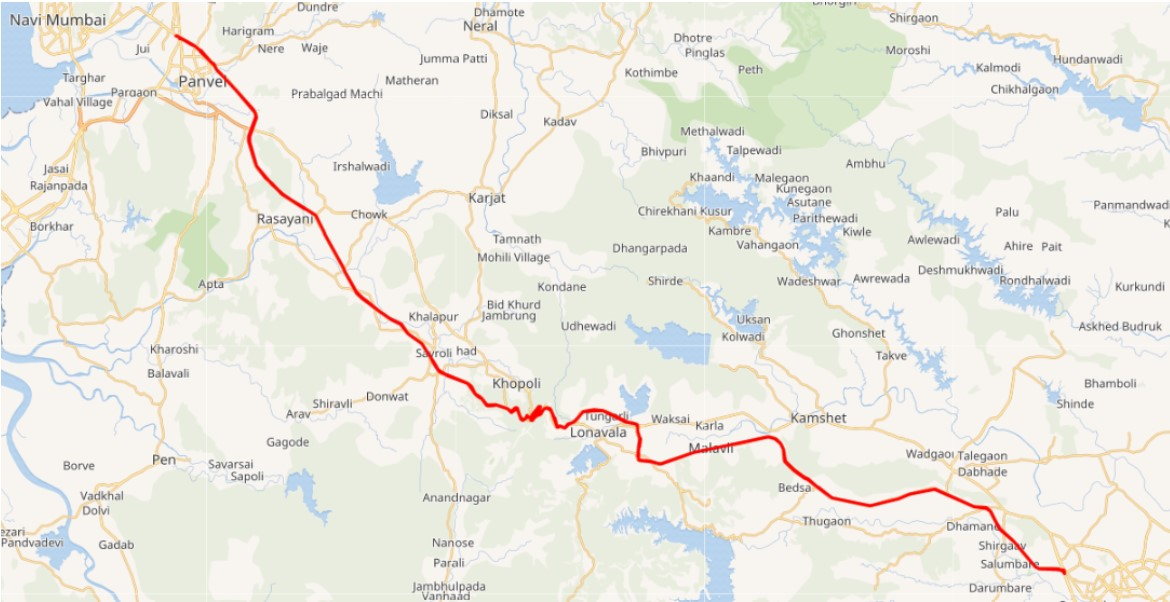
\includegraphics[width=400pt,height=300pt]{pune-mumbai.jpg}
	\caption{Pune-Mumbai Expressway (Existing Map)}
\end{figure}
% \begin{figure}[htbp]			% Sample figure 
% \begin{center}
% \input{pune-mumbai.jpg}			% Be sure to have the input file in the directory
% \caption{}
% \end{center}
% \end{figure}

\newline \newline
\text{The Steps involved in Route Alignment Optimization are as follows:}
\section{Land Use Land Cover Classification}
\text{The Sentinel-2 image of the study area is processed and land use land cover analysis is performed to identify different geological parameters in the region. It involves preparing the thematic layers involving various factors such as: land use, forest cover, soil, slope, aspect, drainage etc. important for determining the optimal route alignment.
\newline
Firstly, the LULC analysis is performed covering 6-7 LULC categories involving road, water body, built up area, forest, river sediments, agricultural land, plantation/man made forest. LULC classification is performed using Deep learning and Machine learning based classifiers such as - Support Vector Machine, Random Forest, K-Means Clustering and Maximum Likelihood Classifiers. The dataset used for training the models is derived from Kaggle for initial training purposes due to time constraints[Dataset] which consists of [] images and classifies the input image into [] classes. \newline
Further, the slope map of the region is prepared using the digital elevation model (DEM) datasets generated from the Survey of India (SOI) topographic map. Slope map is used to determine the flatness of the region for suitability of road construction and can also be classified into classes to depict variations in the region involved. The aspect map prepared from the slope map is used to determine the direction of the slope in the region required mainly for the vertical alignment of the routes.
\newline
Furthermore, soil, drainage and geology maps can also be developed as an improvement to consider the environmental and social aspects of road construction as well as the safety of the route. Soil map gives soil distribution of the region which helps to identify the soil type and its use in agriculture purposes or construction. Geology maps help to determine safety of the routes constructed to predict the possibility of landslides or disasters in or after the road construction. Drainage maps serve an important purpose to determine water bodies and rivers in the region hence, to minimize cost of construction as well as environmental losses.
\newline
Hence, after these series of image processing steps are performed on the input satellite image, we get an output image depicting various geological parameters of the region which can be utilized for further weight ranking and optimization.

}
\section{Weight Assignment and Ranking of the factors}
\text{
In this step, Multi Criteria Decision Making (MCDM) techniques are used to determine relative importance of different factors involved in alignment of routes. Initially, the factors involved in construction classified broadly as economical, social, environmental, geometrical and utility factors are decided by the stakeholders and weight assignment is performed considering the alignment requirements.
\newline
6 weighting methods are implemented and applied on the factors including: AHP (Analytical Hierarchy Process), ANP(Analytical Network Process), Rank Sum, Rank Reciprocal, Rank exponent, Ratio estimation techniques. Different techniques are applied simultaneously to assign weights to the parameters in the most optimal ways without bias and considering all the costs involved. 
\newline
AHP gives most accurate results by scaling the weights of parameters by constructing a pairwise comparison matrix. Two factors are compared at a time in terms of their relative importance to the given objective and then the module calculates a set of weights that give a consistency ratio. The weights are assigned to the parameters optimally and an importance matrix is constructed. The direction map can be constructed using the importance matrix for the given region by assigning weights to the parameters in the region.
\newline
Finally, we get the direction map of the region as the output involving weights assigned to the parameters and classified into different classes according to parameter weights, which is then utilized in the route optimization step.
}

\section{Route Alignment Optimization}
\text{
In this step, which is the final step of route alignment, the region between the 2 cities (in our case- Pune and Mumbai) is searched for an optimized route or path connecting them, considering the relative importance of the parameters as well as constraints involved. The constraints are determined for road construction considering the stakeholders and cost functions involved, some of which include: minimizing the drainage region, wet land and alluvial soil region in construction, minimize regions occupied by communities, forest areas etc. More constraints can be determined for further improvement of the alignment optimization process. 
\newline
Initially, the weight map of the input region is constructed utilizing the direction map and importance matrix, and weight is assigned to each pixel of the region considered according to its relative importance.
\newline
Further, the optimal route search is performed between the source and destination locations, involving weights as the costs of the paths using different search algorithms such as: Dijkstra’s algorithm Bellman Ford algorithm, AI based algorithms - A star, Least Cost Path, Fuzzy logic based algorithms and Genetic Algorithms with Swarm intelligence. Some techniques such as Rank sum and Rank exponent can also be used to find optimal route(s) between start and end locations. Also, ArcGIS based tools such as Spatial Analyst Module can also be used to find optimal alignment directly by giving input as the direction map in the raster form.
\newline
After comparing different algorithms and their outputs, Genetic algorithms using Swarm intelligence based optimization gives most accurate results, with lesser time complexity and can be used effectively for route alignment optimization.
}
%Th is is a section. We can cite a reference like this: \cite{INTERNET} 	
						% Citation. See references.tex for the entry.
% \subsection{Vorpal blade}
% And this is a subsection.
	
% \subsubsection{Tumtum tree}
% You get the drift \ldots
		
% \section{Jubjub Bird}

% \begin{figure}[htbp]			% Sample figure 
% \begin{center}
% %\input{fig1.latex}			% Be sure to have the input file in the directory
% \caption{A simple figure: Square}	% This will appear in the list of figures
% \label{circle}
% \end{center}
% \end{figure}

%_____________________________________________________________________________________________ 
